\documentclass[a4j,11pt,report]{jsbook}
\usepackage[dvipdfmx]{graphicx}
\usepackage{tabularx}
\usepackage{fancybox}
\usepackage{ascmac}
\usepackage{amsmath,amssymb,amsthm}
\usepackage[dviout]{graphicx}
\usepackage{subcaption}
\setlength{\topmargin}{-1in}
\addtolength{\topmargin}{5mm}
\setlength{\headheight}{5mm}
\setlength{\headsep}{0mm}
\setlength{\textheight}{\paperheight}
\addtolength{\textheight}{-25mm}
\setlength{\footskip}{5mm}

\newcommand{\frontpage}[3]{%
\title{卒業論文\\ \vspace{3em}\\{\huge #1}\\ \\#2\vspace{15em}}%
\author{{\huge 成蹊大学理工学部情報科学科}\\ \\{\huge #3}}%
\date{}
\maketitle
\clearpage
\thispagestyle{empty}

\clearpage
}



\newcommand{\point}[1]{
\begin{itembox}[l]{ポイント}
  #1
\end{itembox}
}

\begin{document}

\frontpage  % 以下の各項目を自分のテーマにあわせて修正する.
{計算問題の特徴分布に基づく類題選出による自己学習支援}
{Self Learning Support by Automatic Selection of Calculation Exercises based on Feature Distribution of Exercises}
{S152114 宮地 雄也}

\chapter*{要旨}
\thispagestyle{empty}
\point{
序論と結論の内容をもとに研究の内容をまとめる.
\begin{itemize}
  \item 問いは何か??
  \item 主張は何か??
  \item 結果はどうだったのか?
  \item 得られた成果の意義は?
\end{itemize}
}

\tableofcontents
\thispagestyle{empty}
\clearpage
\thispagestyle{plain}
\setcounter{page}{1}

\chapter{序論 \label{ch:introduction}}

\point{
問題提起を行う.
解く価値があり,簡単には解けず,誰も解いていない問題を扱っていることがわかるようにする.
\begin{itemize}
  \item どういう問題に取り組んだのか?
  \item その問題を解くことがなぜ重要なのか? 社会的意義(有用性)・学術的意義(問題の面白さ)
  \item その問題はどこが難しいのか? なぜこれまで解かれていなかったのか? これまではどうしていたのか?
  \item その問題をどのようなアプローチで解こうとしたのか? なぜそうしたのか?
\end{itemize}
}

昨今,小・中学生の理系離れが問題視されている.平成30年度全国学力・学習状況調査(全国学力テスト)の結果では平均正答率は小学校では算数Bが51.7\%,中学校数学では47.6\%とどちらも最も低く,ついで国語,理科の順で正答率が低く,結果として理系教科の習熟度が低いことを示している.
この要因の一つに,数学は一つの計算方法が様々な分野に横断していくことが一度,苦手を生んでしまったらそこからの分野の理解度が下がり,次の分野での応用がきかないために連鎖的に苦手を増幅するように思う.各単元のちょっとした積み残しが,後々,尾を引いていることが全国学力テストの結果から見て取れる.この状況を打破するには子供一人一人の苦手と向き合い,苦手と感じる前に理解していくしかない.
しかしながら,生徒と向き合うべき教師の労働時間は,...<悪さについてノベル>

この打開策として,Edtech(エドテック)に期待が集まっている,
<いいことつらつら>
その中でも,生徒一人一人に対し,最適な学習を提供するAdaptive Learning(アダプティブラーニング)に可能性を感じた.
これを数学教育で効果的に用いれれば,つまずく子供を減らせるのではないかと考えた.
しかし,教育の情報は,生徒の情報と結びついているためオープン化できないという問題がある.
また数学の苦手に対してどのような手法を用いれれば効果的なのかも未だ模索中である.

そこで計算式自体の特徴を抽出し,間違えた問題と同様の特徴を持つ問題が復習する類題として最適なのではないかという仮定のもと,本論文では数式の特徴を掴むために自然言語処理の分野で使用される分散表現を適用し,さらに再起ニューラルネットワークを用いて数式ベクトルを作り出すことを目標とし,そのベクトルを用いて実際に復習問題生成を行った.


\section{memo}
近年,子供達一人一人に目を向けたアダプティブラーニングが注目を集めていますが,現在の日本の教育現場では集合教育が基本であり
一人一人に対応するのは難しい.また教員の働き方にも是正が求められていて,仮に個々に対応しようとすると労働時間外になってしまう.
そこで個人最適化した学習を情報技術で叶えようとする動きが活発である.
そこで私は間違えた問いに対して復習問題を出す際,その数式の特徴を捉えて類題が作れないかと考えた.
今までは問題をといた子供達の集合に目を向けられていたが,本論文では数式自体に目を向け類似する問題を作り出そうとした.
本論文では数式の特徴を掴むために自然言語処理の分野で使用される分散表現を適用し,さらに再起ニューラルネットワークを用いて数式ベクトルを作り出すことを目標とし,そのベクトルを用いて実際に復習問題生成を行った.




\chapter{背景知識\label{ch:background}}

\point{
以降の内容を理解するための準備を行う.
\begin{itemize}
  \item 章題は適切なものに変えること.章をわけてもよい.
  \item 以降の説明で用いる専門用語・表記法を説明する.
  \item 以降の内容を理解するのに必要となる,技術や理論を説明する.
\end{itemize}
}


\section{アダプティブラーニング}

*******************************************

今世の中でどのようなことが行われているかを収集.
その手法を2,3事例あげて説明

*******************************************

アダプティブラーニングとは、学習者一人ひとりの学習進捗度(学習進度)に最適化された学習方法と学習教材を選択し、
提供する仕組みを持つ学習エンジンやシステム、ソフトウェア、サービスなどを統括的に指す言葉です。

アダプティブラーニングは、IT技術を教育分野に活用するEdTech(Education Technology)の1つとして世界中から多くの注目を集めています。
アダプティブラーニングの先駆企業であり世界中でシェアを獲得している米Knewton社CEOのライアン・プリチャード氏は、日本法人であるニュートンジャパン株式会社主催のアダプティブラーニングをテーマにしたイベント『Knewton Day Tokyo 2017- Adaptive Learning Summit -』のQ&Aセッション内で、アダプティブラーニングの定義について上記のように回答しました。
よって本論文中でも以下のように定義する.
\begin{quote}
  データをもとにパーソナライズされた経験を継続的に提供するもので、
  生徒がシステムを使うたびにコンテンツやモデルをアップデートし、最適な道筋をアップデートするもの
\end{quote}

日本国内での様子..


\section{分散表現}
様々な手法を紹介する
CBow,skipGram,GloVeなど
計算式を並べて最後にどこが長所で,どこが違うのかを表現


\section{LSTM(Long short-term memory)}

通常のRNNでは叶わないところを明確に

\section{Attention}

これからね



\chapter{提案手法(章題は変える)\label{ch:method}}
\point{
自分の提案する解決方法を説明する.
\begin{itemize}
  \item 章題は適切なものに変えること.章をわけてもよい.
  \item 必ず具体例を用いること.
  \item 最初に問題を解く上で最も難しい点とそれを解決するアイデアを示す.
  \item 詳細については,全体の流れを示した後,各ステップについて説明する.
  \item 検討時に行った予備評価の結果があれば示す.
\end{itemize}
}

\section{システム全体の流れ}
<図をいれながら>



\section{計算式の特徴量抽出}
\subsection{概要}
<idea>
(内容充実させる)
数式を分布化する際,そのベクトルの中に数式の特徴を入れ込んだベクトルを生成する手法が確立していない.そこで本論文では数式の各文字,記号を単語のようにみなし,onehotベクトルを作成し,それを埋め込み層で特徴を踏まえた低次元ベクトルに変換したのち,系列変換モデルで読み込むことで低次元で数式の特徴を掴んだベクトルを生成できないかと考えた.

<手法>
この考えを実現するために数式は我々が目にする$2x+3=5$, $\frac{3x-1}{2}+4=\frac{2}{5}$ではなく,テキスト化かつその特徴を強く受けた形に変換する必要がある.
そこで本論文では数式をある一定のルールの中でテキスト化されている{\TeX}形式の数式を用いる.
上記の計算式なら\verb#2x+3=5#,\verb#\frac{3x-1}{2}+4=\frac{2}{5}#とし,このテキストデータを用いて文字単位の埋め込んだベクトルを作成する.

実験を行った手法は以下の三種法で行い,それぞれ分布をpythonを用いて確認した.
\begin{itemize}
  \item CBOW
  \item SkipGram
  \item ...
\end{itemize}

onehotベクトルの置き方は
\begin{itemize}
  \item $[0,1,2, ... ,9,+,-,=,x ...]$ のように各数字,各記号に割り当てる方法
  \item 出てきた数字,数式の塊をonehotを置く方法($[0,1,2, ... 3.6,0.11,...=.+,-]$)
  \item 3桁までの数字,数式に現れる記号
\end{itemize}


\subsection{文字分布の入手}
予備実験として文字の分布を入れる
CBOW,SkipGram,(できれば groveも)

できればベクトルの足し引きとかできればword2vecの論文にもそうので結果を確かめたい.



\begin{figure}[ht]
  \begin{minipage}
    \begin{figure}[ht]
      \begin{center}
        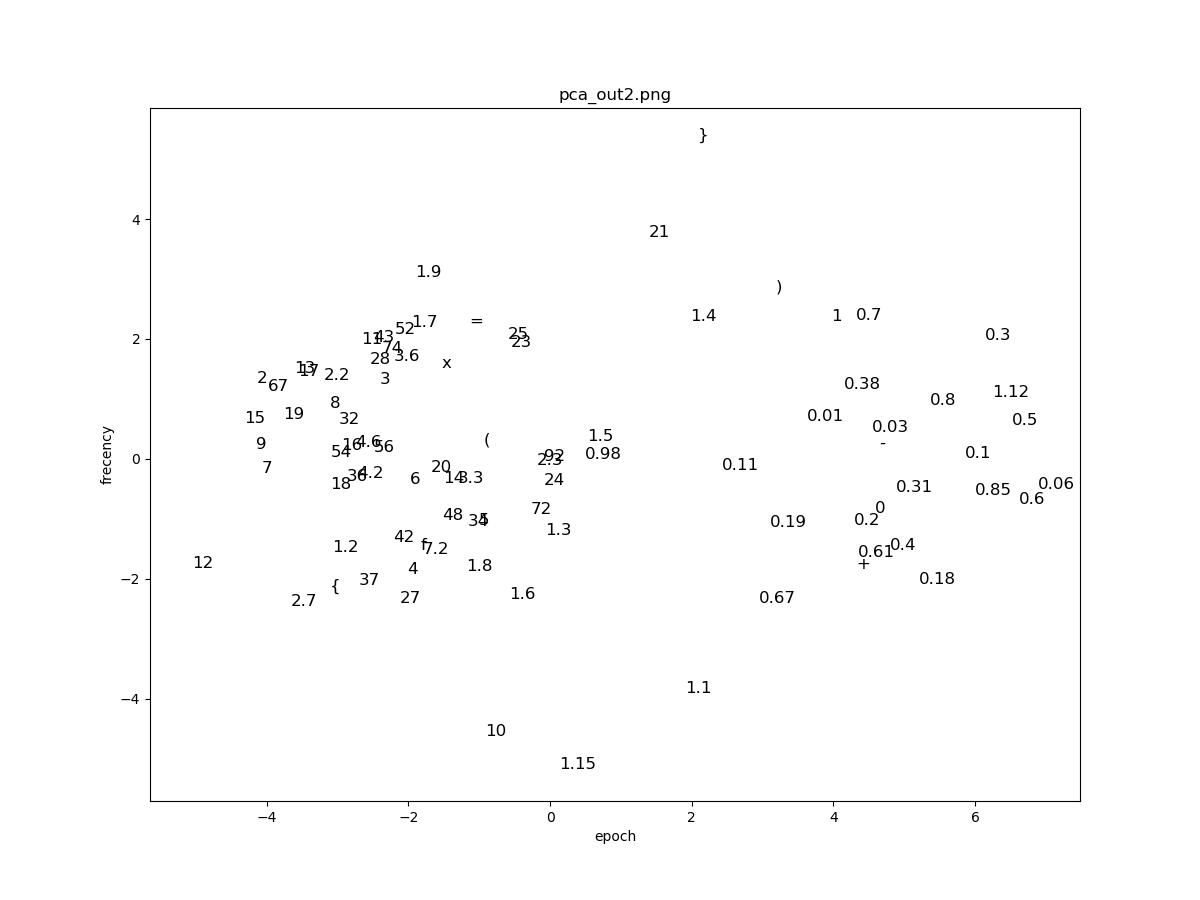
\includegraphics[width = 10cm]{image/pca_out2.png}
        \caption{pcaでのCBOWを用いた文字分布}
        \label{fig:pca_out2}

      \end{figure}

      \begin{figure}[ht]

        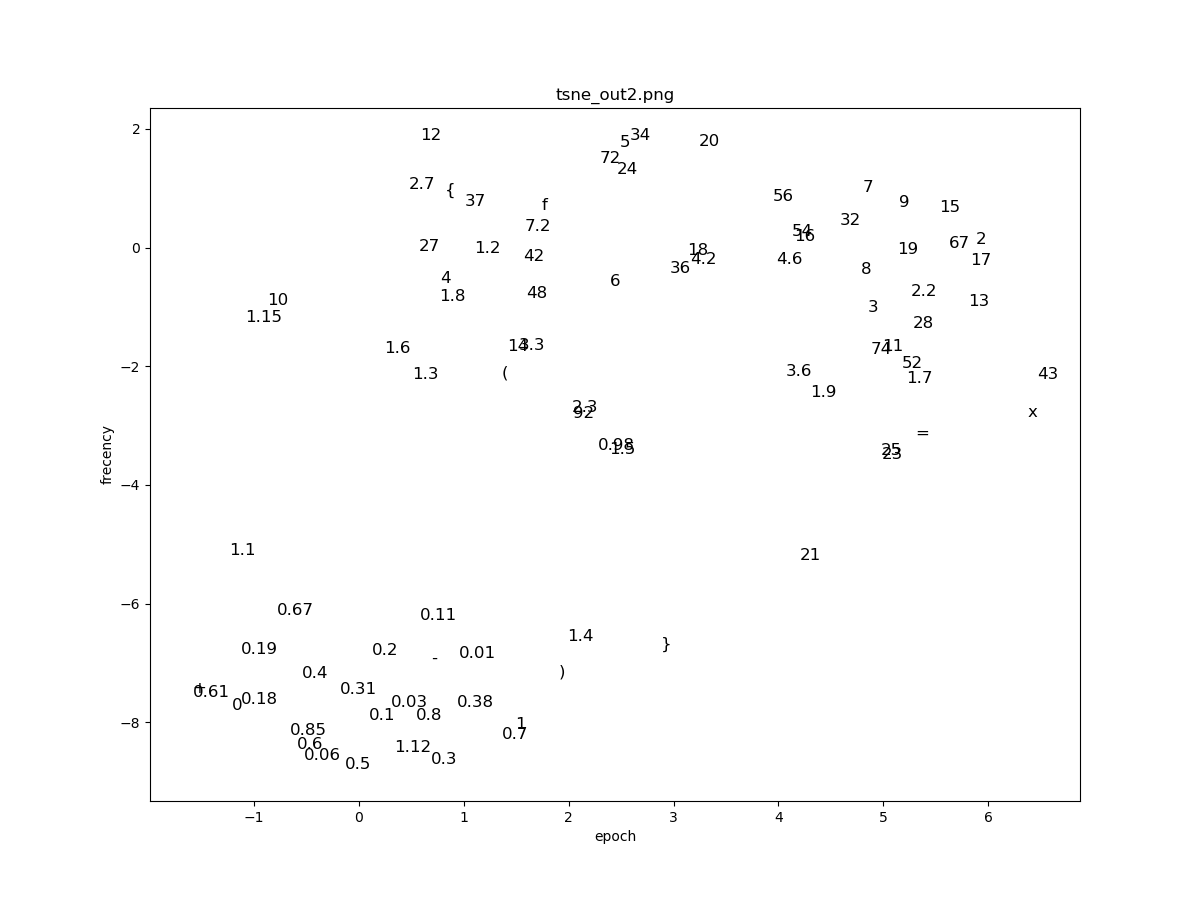
\includegraphics[width = 10cm]{image/tsne_out2.png}
        \caption{tーsneでのCBOWを用いた文字分布}
        \label{fig:tsne_out2}
        
      \end{center}

    \end{figure}
  \end{minipage}

\end{figure}



<おまけだからさらっと>
\section{判定機}
今回提案するシステムではといたプリントを読み込みその結果を判別して間違った計算問題を見つけ,その類題を選出する.
\subsection{概要}

\begin{figure}[ht]
  \begin{center}
    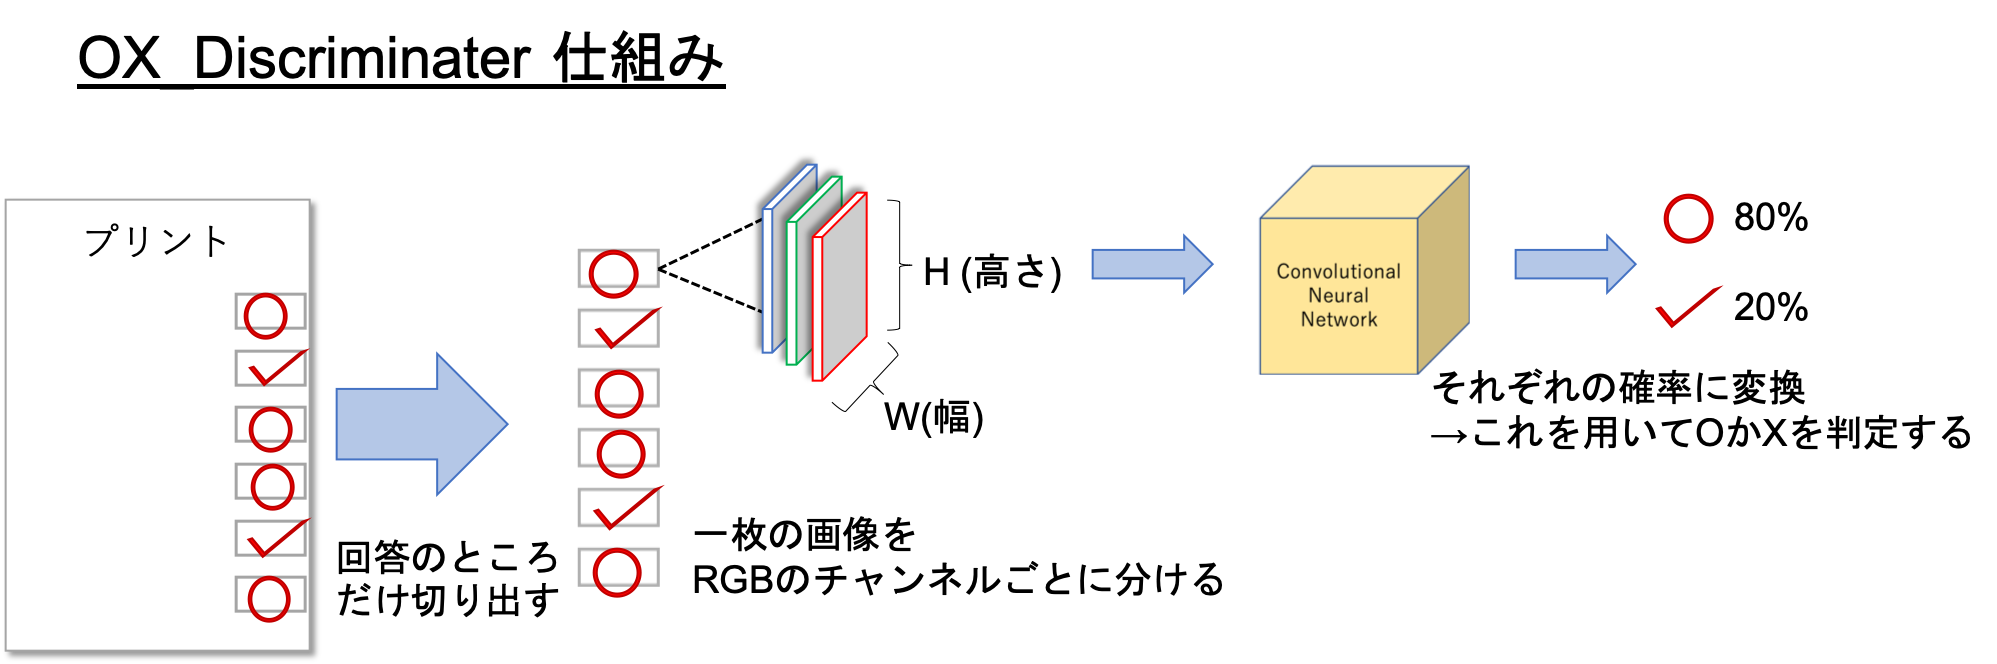
\includegraphics[width = 15cm]{image/OX_Discriminater.png}
    \caption{OX_Discriminaterイメージ図}
    \label{fig:OX_Discriminater_image}
  \end{center}
\end{figure}

『文章で説明』

\begin{figure}[ht]
  \begin{center}
    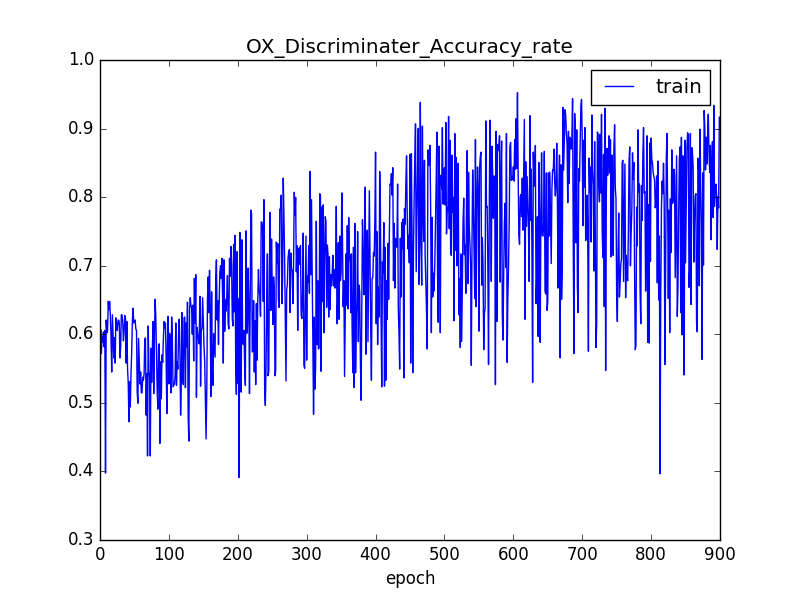
\includegraphics[width = 10cm]{image/OX_Discriminater_Accuracy_rateplot.png}
    \caption{学習の様子}
    \label{fig:OX_AccRate}
  \end{center}
\end{figure}

→ あと誤差も(データ取り直しています)

\clearpage










\chapter{結果とその検討 \label{ch:result}}

\point{
自分の提案する方法が序論で提起した問題を解決できているかを評価・分析する.
\begin{itemize}
  \item 目的.何を確認するためのものか
  \item 方法.そのためにどういう実験を行ったか? 実験環境・用いたデータとその選定理由・手順を示し,評価の適切性を論証すること.
  \item 結果.その結果はどうだったか? 表やグラフを用いてまとめる.表はTeX,グラフはexcelでなくpythonを用いて作成すること.
  \item 分析.その結果から何が言えるか? 達成できた点・不足している点を理由と共に述べ,原因を考察する.
\end{itemize}
}
\section{実験}
\subparagraph{計算式の特徴量抽出}
\begin{itemize}
  \item 目的.数式のベクトル表現は可能なのかどうか
  \item 方法.埋め込み層,ネットワーク構成を変えながらEncoder-Decoderで復元を試みる
  そのEncoderの出力値を数式ベクトルとしてみなし,pca,T-sneで二次元ベクトルに圧縮し図示する
  \item 結果.これから
  \item 分析.これから
\end{itemize}

\subparagraph{計算式の特徴量からの類題選出}
\begin{itemize}
  \item 目的.求めた計算式のベクトルから特徴を捉えた数式を選出できるか
  \item 方法.特徴量ベクトルからk近法で選出,ある生徒の間違えた一問から類題を選出し,実際にその問題を間違えていたかを確認,また,逆にあっていた問題からも同様な手法で確認
  \item 結果.これから
  \item 分析.これから
\end{itemize}
\section{評価}
\section{分析}
\section{検討}





\chapter{関連研究\label{ch:relatedwork}}
\point{
この研究に関連する他の研究を紹介し,この研究との違いを明確にする.
\begin{itemize}
  \item 文献は「Mnihらは~という手法を提案している\cite{Mnih15}.」のように\texttt{cite}コマンドを用いて文献番号を示すこと.
  \item 2ページ以上書く.
\end{itemize}

https://code.google.com/archive/p/word2vec/

https://techblog.asahi-net.co.jp/entry/2018/10/05/180310
}

\chapter{結論と今後の課題 \label{ch:conclusion}}

\point{
序論で提起した問いとそれに対する答えをまとめる.
\begin{itemize}
  \item 提案手法のアイデアおよび評価結果を振り返る.
  \item この研究で得られた知見をまとめる.
  \item 今後の課題について述べる.
\end{itemize}
}

\bibliographystyle{ipsjsort}
\bibliography{ref}

\appendix

\chapter{形式上の注意}

\begin{itemize}
  \item 文字コードはUTF-8に統一する.
  \item 論文ファイル名は\texttt{chishiro-thesis.tex},文献ファイル名は\texttt{chishiro.bib}のように名前\texttt{-thesis.tex}とする.
  \item 句読点は全角のカンマ,ピリオドを用いる.
  \item 英数字はすべて半角を用いる.ギリシャ文字は{\TeX}の定義を用いる.$\alpha, \beta, ...$
  \item カンマの前にはスペースを入れず,カンマの後はスペースをひとつ入れる.
  \item 数式は{\TeX}の数式機能を用いる.例: $x^2$,\[f(x) = x^2 + 2x + 1.\].
  \item プログラムテキストはタイプライターフォントを用いる(例: \texttt{hello}).
  \item 文章構成(章・節・小節・箇条書き)は{\TeX}の機能を用いて指定する.自分で見出しなどを作らない.
  \item 題目には研究目的・方法・対象を特徴づける情報を入れる.
  \item 図のタイトルは図の下,表のタイトルは表の上に書く.
  \item 図表番号の参照は\verb#\label#および\verb#\ref#を用いる.自分で図表番号を指定しない.
  \item 表は{\TeX},グラフはすべてpythonで作成する.
  \item 図表番号のない図は用いない.
  \item 参照の?は必ず取り除く.
  \item 段落は意味の区切りでわける.意図しない字下げが入った場合\verb#\noindent#を用いて修正する.
  \item 参考文献は10以上あげる.
\end{itemize}


\chapter*{謝辞 \label{ch:acknowledgement}}
\thispagestyle{empty}
\point{
本のあとがきに相当する部分.半ページ以上書く.
卒業研究に協力者してくれた方々へのお礼を忘れずに述べる.
}


\end{document}
